\section{Challenges: Testing Internal and Network Nondeterminism}
\label{sec:challenge}
To illustrate the challenges in testing networked applications, we discuss two
features of \http---conditional requests~\cite{rfc7232}
and message forwarding~\cite{rfc7231}---showcasing internal nondeterminism
and network nondeterminism, respectively.
%% \hzh{we should make sure we always use either internal/external or
%% internal/network. in particular, the 3rd contribution uses internal/external,
%% while everywhere else seems to use internal/network.}

\paragraph*{Internal Nondeterminsm}
\http requests can be conditional: if the client has a local copy of some
resource and the copy on the server has not changed, then the server needn't
resend the resource.  To
achieve this, an \http server may generate a short string, called an ``entity tag'' (ETag), identifying the
content of some resource, and send it to
the client: %% \bcp{Make the font a bit smaller}
\begin{lstlisting}[style=customc]
/* Client: */
GET /target HTTP/1.1

/* Server: */
HTTP/1.1 200 OK
ETag: "tag-foo"
... content of /target ...
\end{lstlisting}
The next time the client requests the same resource, it can include the ETag in
the GET request, informing the server not to send the content if its ETag
still matches:

\begin{lstlisting}[style=customc]
/* Client: */
GET /target HTTP/1.1
If-None-Match: "tag-foo"

/* Server: */
HTTP/1.1 304 Not Modified
\end{lstlisting}
% The server compares the request's ETag with that stored for the target
% resource.
% If matched, the server responds with code 304 and the client knows the
% target's
% content has not changed from the previously sent content.
If the tag does not
match, the server responds with code 200 and the updated content as usual.
%
Similarly, if a client wants to modify the server's resource atomically by
compare-and-swap, it can include the ETag in the PUT request as \inlinec{If-Match} precondition, which
instructs the server to only update the content if its current ETag matches.
% \begin{lstlisting}[style=customc]
% /* Client: */
% PUT /target HTTP/1.1
% If-Match: "tag-outdated"
%
% /* Server: */
% HTTP/1.1 412 Precondition Failed
% \end{lstlisting}
% The server compares the request's ETag with the target's.  If they don't match
% (indicating the client has an outdated version of the target resource), the
% server does not process the modification, and responds with code 412.  Only if
% the client provides a matching ETag does the server update the target's content
% per requested.  A pseudocode for this compare-and-swap logic is shown in
% \autoref{fig:if-match-model}.

\ly{This is a good example, but how general is the
  problem, since one might question the popularity of ETags? On the other hand,
  if your testing framework targets application layer protocols rather than just
  HTTP, maybe there are more similar examples? For example, file/mail servers or
  databases might also require some synchronization mechanisms similar to
  compare-and-swap? And there might be other examples that's not
  compare-and-swap?}\bcp{Agree that this is important to discuss.}
  \lys{Mentioned at the end of this section.}

Thus, whether a server's response should be judged {\em valid} or not
depends on the ETag it generated
when creating the resource.  If the tester doesn't know the server's internal
state ({\it e.g.}, before receiving any 200 response including the ETag), and
cannot enumerate all of them (as ETags can be arbitrary strings), then it needs
to maintain a space of all possible values, narrowing the space upon further
interactions with the server.
% ~\ly{If I understand it correctly, the
%   non-determinism mostly comes from the fact that the algorithm to generate
%   ETags is unknown and depends on a lot of server's internal states---the fact
%   that the server supports ``compare and swap'' seems less relevant? If so, I
%   think this subsection should focus more on where the non-determinism comes
%   from, and why this makes it hard for testers, rather than demonstrating how
%   HTTP/1.1 implements ``compare and swap''.}\bcp{I agree---the whole
%   compare-and-swap discussion could be reduced to a sentence.  I'll make
%   this fix.}

It is possible, but tricky, to write an ad hoc tester for \http by
manually ``dualizing'' the behaviors described by the informal specification
documents (RFCs).
The protocol document describes {\em how} a valid server should handle
requests, while the
tester needs to determine {\em what} responses received
from the server are valid.  For example, ``If the server has revealed some
resource's ETag as \inlinec{"foo"}, then it must not reject requests targetting
this resource conditioned over \inlinec{If-Match: "foo"}, until the resource has
been modified''; and ``Had the server previously rejected an \inlinec{If-Match}
request, it must reject the same request until its target has been
modified.'' \autoref{fig:etag-tester} shows a hand-written tester for
checking this bit of ETag functionality; we hope the reader will agree that
this testing logic is not straightforward to derive from the informal
``server's eye'' specifications.

\paragraph*{Network Nondeterminism}
%% \lys{Network nondeterminism seems more important as a contribution, but internal
%%   nondeterminism were discussed much more.}\sz{Maybe drop the subsection and
%%   call out ``internal'' vs. ``network'' nondeterminism via paragraphs
%%   instead?This discussion is still focused on HTTP/1.1, so they belong
%%   together?}
%% \bcp{Changed to paragraph.}

When testing an \http server over the network, although TCP preserves message
ordering within each connection, it does not guarantee any order between
different connections.  Consider a proxy model in \autoref{fig:proxy-model}: it
specifies {how} a server should forward messages. \bcp{I don't
  understand why we are talking about proxies here: a simple ``server +
  several clients'' situation is enough to create network nondeterminism.  (I
would expect that proxying might create {\em additional} possibilities for
nondeterminism, of course.)  \lys{We need to talk about proxy somewhere, and I
  didn't find a good place elsewhere.}}  \bcp{Moreover, the more I look at
  figures 2--5
the more confusing I find them.  Only figure 5 mentions connections, but ---
for example, in figure 3, if
we assume just a single connection between the observer and the proxy and a
single connection from the proxy back to the observer, then the reordering
shown in the figure is NOT valid.  \lys{Updated figure.  No proxy uses the same
  connection for multiple requests.  The proxy never knows if there's a next
  request that can use the same connection.}}
%% \bcp{Confusing: ``Servers'' do not normally forward messages---they just
%%   handle them.  \lys{I chose proxy rather than other parts of HTTP: We need
%%   to introduce proxy somewhere, and discuss network nondeterminism somewhere,
%%   so better both in here.}}
When the forwarded messages are scrambled as in \autoref{fig:proxy-valid-trace},
the tester should be {\em loose} enough to accept the server, because a valid
server may exhibit such reordering due to network delays.  The tester should
also be {\em strict} enough to reject a server that behaves as
\autoref{fig:proxy-invalid-trace}, because no network delay can let the proxy
forward a message before the observer sends it.

\iffalse
Similar reorderings can arise from the server's runtime environment: To
handle multiple clients, it is natural
to write a server that runs multiple threads concurrently, and the operating
might schedule these threads nondeterministically.  Moreover, the OS itself
might reorder messages sent and received on different TCP channels.
When testing the server over
the network, such nondeterminism outside the code of the server program but
still within the machine on which the server is executing is indistinguishable
from nondeterminism
caused by network delays, and is thus covered by the concept ``network
nondeterminism.''
\fi

The kinds of nondeterminism exemplified here can be found in many other
scenarios: (i) Servers may use some (unknown) algorithm to generate internal
state for nonces, sequence numbers, caching metadata, {\it etc}, featuring
internal nondeterminism.  (ii) When the server runs multiple threads
concurrently ({\it e.g.} to serve multiple clients), the operating system might
schedule these threads nondeterministically.  When testing the server over the
network, such ``nondeterminism outside the code of the server program but still
within the machine on which the server is executing'' is indistinguishable from
nondeterminism caused by network delays, and thus can be covered by the concept
``network nondeterminism.''

% Upon interacting with the server, our tester needs to reason about possible network
% delays, and find a corresponding server-side behavior that matches the
% interaction.

\section{Specification Language}
\label{sec:spec-language}
A specification in our framework consists of two parts: a server model
specifying
server-side behavior,\bcp{there was a discussion of this somewhere else:
  isn't our ``application model'' here just specifying HTTP and WebDAV? And
  so isn't it also generic?  \lys{Not generic over all L7 protocols.}}
and a network model describing network
delays.  By
composing these two models, we get a tester-side specification of valid
observations over the network.

Formally, our specifications are written as {\em interaction trees}, a generic
data structure for representing interactive programs in Coq.  This language
allows us to write rigorous mathematical specifications, and transform the
specification into tester conveniently.  In this
paper, we present models as pseudocode for readability.  Technical details
about interaction trees can be found in \cite{itree}.

\autoref{sec:app-model} shows how to handle network nondeterminism.
\autoref{sec:symbolic-model} then expands the model to address internal
nondeterminism.

\subsection{Server and Network Models}
\label{sec:app-model}

%% \bcp{This subsection is called Application Model, but it spends most of its
%%   time motivating the network model...}

The {\em server model} specifies how the server code
interacts with the network interface.  For example, an extremely simplistic model of
an HTTP proxy\bcp{again, it feels like proxies are coming out of nowhere
  \lys{I'll try to make proxy more like a part of HTTP than an extension.}}
(shown in \autoref{fig:proxy-model}) is written as:

\begin{figure}
  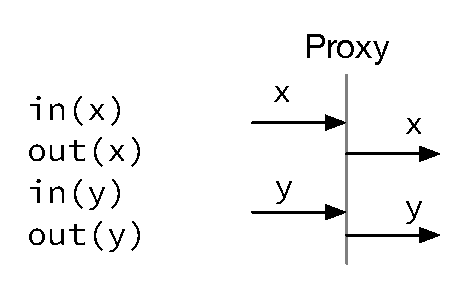
\includegraphics[width=0.4\linewidth]{figures/proxy-linear}
  \caption{Proxy model specifying a server that forwards a message immediately
    upon receiving it.}
  \label{fig:proxy-model}
\end{figure}

\begin{figure}
  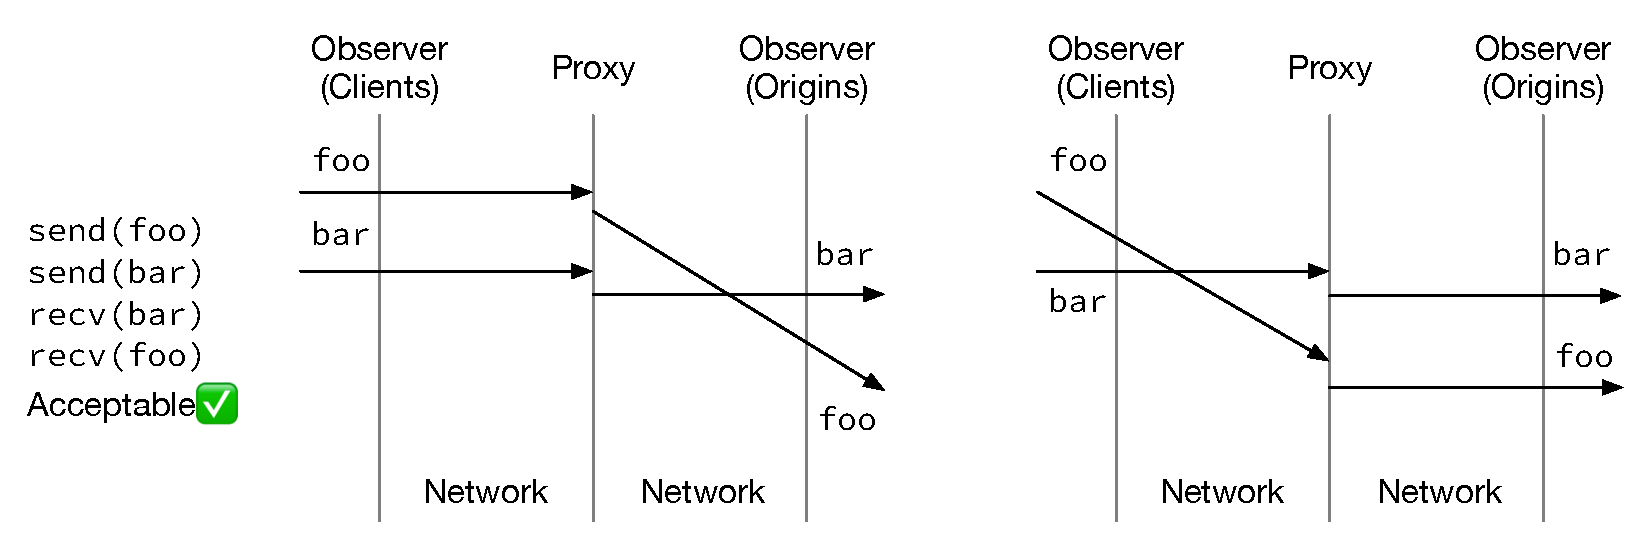
\includegraphics[width=\linewidth]{figures/proxy-valid-trace}
  \caption{A reordered observation, with two valid network-level explanations.}
  \label{fig:proxy-valid-trace}
\end{figure}

\begin{figure}
  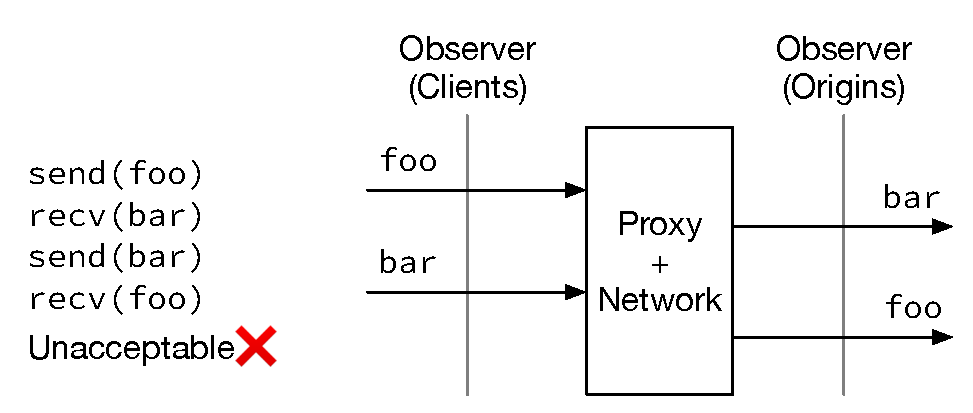
\includegraphics[width=0.7\linewidth]{figures/proxy-invalid-trace}
  \caption{Example of invalid observation.}
  \label{fig:proxy-invalid-trace}
\end{figure}

\begin{lstlisting}[style=customcoq]
let proxy() =
    msg := recv();
    send(msg);
    proxy()
\end{lstlisting}

An implementation is said to be {\em valid} if it is indistinguishable from
the model when viewed from across the network.  Consider
the following proxy implementation that reorders messages:
%% \bcp{We need a way of better distinguishing models from implementations,
%%   e.g. a naming convention that will make clear which is which.  ``proxy''
%%   and ``proxy\_reorder'' sound like they could be either.}
\bcp{Why are we suddenly switching to C syntax??  \lys{To distinguish
    implementation from specification.}}

\begin{lstlisting}[style=customc]
  void proxy_implementation() {
    while (true) {
      recv(&msg1); recv(&msg2);
      send(msg2);  send(msg1);
    }
  }
\end{lstlisting}
This reordered implementation is valid, because the model itself may
exhibit the same behavior when observed over the network, as shown in
\autoref{fig:proxy-valid-trace}.  This ``implementation's behavior is
explainable by the model, considering network delays''
relation is called {\em network refinement} by
\textcite{cpp19}.
%% \bcp{This doesn't sound right: refinement should be an
%%   asymmetric relation, but indistinguishability shoud be symmetric.}

To specify network refinement in a testable way, we introduce
the {\em network model}, a conceptual implementation of the transport-layer
environment between the server and the tester.  It models the network as a
nondeterministic machine that absorbs packets and,  after some time, emits
them again.  \autoref{fig:tcp-model} shows the network model for concurrent TCP
connections: The network
either
receives a packet from some node, or sends the first packet en route of some
connection.  This model preserves the message order within each connection,
but it exhibits all possible reorderings among different connections.

\begin{figure}
\begin{lstlisting}[style=customcoq]
let tcp (buffer : list packet) =
    let absorb =
        pkt := recv();
        tcp (buffer ++ [pkt]) in
    let emit =
        let pkts = oldest_in_each_conn(buffer) in
        pkt := pick_one(pkts);
        send(pkt);
        tcp (remove(pkt, buffer)) in
    or (absorb, emit)
\end{lstlisting}
\caption{Network model for concurrent TCP connections.  The model maintains a
  \ilc{buffer} of all packets en
  route.  In each cycle, the model may nondeterministically branch to either
  absorb \ilc{or} emit a packet.  Any absorbed packet is appended to the end of
  buffer.  When emitting a packet, the model may choose a connection and send
  the oldest packet in it.
  %% \bcp{What is choose\_connection?? what is a packet?  How do we get from a
  %% packet to a connection?}
}
\label{fig:tcp-model}
\end{figure}

The network model does not distinguish between server and tester.  When one end
\ilc{send}s some message, the network \ilc{recv}s the message and \ilc{send}s it
after some cycles of delay; it is then observed by the other end via some
\ilc{recv} call.

In \autoref{sec:net-compose}, we compose the server and network models to yield an
observer-side specification for testing purposes.

\subsection{Symbolic Representation of Nondeterministic Data}
\label{sec:symbolic-model}

To incorporate symbolic evaluation in our testing framework, our specification
needs to represent internally generated data as symbols.  Consider HTTP
PUT requests with \inlinec{If-Match} preconditions: Upon success, the server
generates a new ETag for the updated content, and the tester does not know the
ETag's value immediately.  Our symbolic model in \autoref{fig:if-match-model}
represents the server's generated ETags as fresh variables.  The server's future
behavior might depend on whether a request's ETag matches the generated
(symbolic) ETag.  Such matching produces a symbolic boolean expression, which
cannot be evaluated into a boolean value without enough constraints on its
variables.  Our model introduces \ilc{IF} operator to condition branches over
a symbolic boolean expression.  Which branch the server actually took is decided
by the derived tester in \autoref{sec:derivation}.

In \autoref{sec:derive-internal}, we implement the symbolic evaluation process
that checks servers' observable behavior against this symbolic model.

\begin{figure}
\begin{lstlisting}[style=customcoq]
(* matches : (etag * exp etag) -> exp bool *)
(* IF      : (exp bool * T * T) -> T       *)
let put (k    : key,
         t    : etag,
         v    : value,
         data : key -> value,
         xtag : key -> exp etag) =
    IF (matches(t, xtag[k]),
    (* then *)
       xt := fresh_tag();
       let xtag' = update(xtag, k, xt) in
       let data' = update(data, k, v)  in
       return (OK, xtag', data'),
    (* else *)
       return (PreconditionFailed, xtag, data))
\end{lstlisting}
\caption{Symbolic model handling conditional PUT request.  The model maintains
  two states: \ilc{data} that maps keys to their values, and \ilc{xtag} that
  maps keys to symbolic variables that represent their corresponding ETags.
  Upon receiving a PUT request conditioned over ``If-Match: \ilc{t}'', the
  server should decide whether the request ETag \ilc{matches} that stored in the
  server.  Upon matching, the server processes the PUT request, and represents
  the updated value's ETag as a fresh variable.
%% \ilc{exp T} is the type of a symbolic expression whose value has type
%% \ilc{T}. \bcp{Put type declarations inline.}  \bcp{What is IF and how does it
%% differ from ordinary if expressions?}
}
\label{fig:if-match-model}
\end{figure}

\section{Derivation: from Server Specification to Testing Program}
\label{sec:derivation}
\begin{figure}
  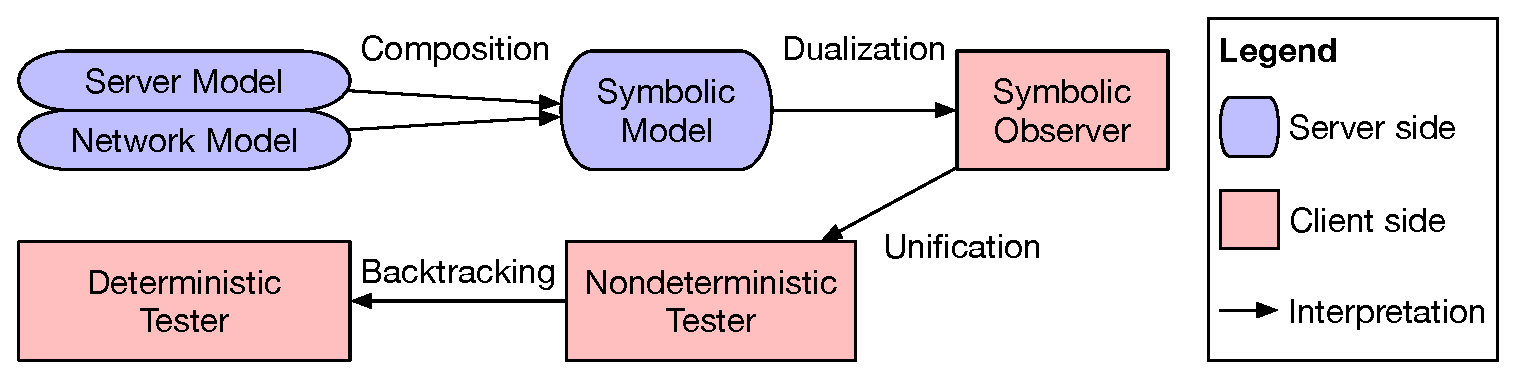
\includegraphics[width=\linewidth]{figures/framework}
  \caption{Deriving tester program from specification}
  \label{fig:framework}
\end{figure}
From the specified the application and network models,
%% \sz{Remind the reader what the L7 and L4 models do, per the comment made
%% later. Also, will the L4 level be shared across many L7 models?},
our framework automatically derives a tester program that
interacts with the server and determines its validity.  The derivation framework
is shown in outline in \autoref{fig:framework}.  Each box is an interaction tree
program, and the arrows are
%% \ly{Maybe this is clear to experts, but I'm not clear what's the
%%   difference between a model program and a reference implementation. Or are they
%%   the same thing?}\bcp{I also don't understand ``model program''}
``interpretors'' that transform one interaction tree into another.
\autoref{sec:interpret} explains the concept of interpretation, and the rest of
this section describes how to interpret the specification into a tester program.
%% \bcp{``instantiating the model's events with specific rules'' doesn't say
%% much to me; hopefully this becomes clearer below, but we should avoid
%% confusing readers here too.}

\subsection{Interpreting Interaction Trees}
\label{sec:interpret}

\begin{figure}
  \begin{lstlisting}[style=customcoq,numbers=right,escapechar=\%]
let acc(sum) =
  x := recv(); send(x+sum); acc(x+sum) in
let tee(m) =
  match m with %\label{line:match}%
  | x := recv(); m'(x) =>
    a := recv(); print("IN" ++ a); tee(m'(a))%\label{line:handler1}%
  | send(a); m' =>
    print("OUT" ++ a); send(a); tee(m') %\label{line:handler2}%
  end in
tee(acc(0))
(* ... is equivalent to ... *)
let tee_acc(sum) =
  a := recv(); print("IN" ++ a);
  print("OUT" ++ (a+sum)); send(a+sum);
  tee_acc(a+sum) in
tee_acc(0)
  \end{lstlisting}
  \caption{Interpretation example.  \ilc{acc} receives a number and returns the
    sum of numbers received so far.  \ilc{tee} prints all the numbers sent and
    received.  Interpreting \ilc{acc} with interpretor \ilc{tee} results in a
    program that's equivalent to \ilc{tee_acc}.}
  \label{fig:logger}
\end{figure}

Interaction tree programs can be destructed into an interaction event followed
by another interaction tree program.  Such structure allows us to {\em
  interpret} one program into another.  \autoref{fig:logger} shows an example of
interpretation: The original \ilc{acc} program sends and receives messages, and
the \ilc{tee} interpretor transforms the \ilc{acc} into another program that
also prints the messages sent and received.

Such interpretation is done by pattern matching on the program's structure in
\autoref{line:match}.  Based on what the original program wants to do next, the
interpretor defines what the result program should do in \autoref{line:handler1}
and \autoref{line:handler2}.  These programs defined in accordance to events are
called {\em handlers}.  By writing different handlers for the events,
interpretors can construct new programs in various ways, as shown in following
subsections.  Further details about interpreting interaction trees are explained
by \textcite{itree}.

\subsection{From Server Specification to Tester Program}
\label{sec:derive-internal}

For simplicity, we first explain how to handle servers' internal nondeterminism
with symbolic evaluation.  This subsection covers a subgraph of
\autoref{fig:framework}, starting with dualizing the symbolic model.
Here we use the server model itself as the symbolic model, assuming no
reorderings by network delays.  We will compose the server model with the
network model in \autoref{sec:net-compose}, addressing network nondeterminism.

\paragraph*{Dualization}
To {\em observe} the server's behavior, we have to interpret the specified
server-side events into tester-side events: When the server should send a
certain message, the tester expects to receive the specified message, and
rejects the server upon receiving an unexpected message; when the server should
receive some message, the tester generates a message and sends it to the server,
as shown in \autoref{fig:sym-observe}.

\begin{figure}
  \begin{lstlisting}[style=customcoq]
let observe (server) =
  match server with
  | pkt := recv(); s'(pkt) =>
    p := gen_pkt(); send(p); observe (s'(p))
  | send(pkt); s' =>
    p := recv(); guard(pkt, p); observe (s')
  | IF (x, s1, s2) =>
    (* Allow validating observation with [s1],
     * provided [x] is unifiable with [true];
     * Or, unify [x] with [false],
     * and validate observation with [s2]. *)
    determine(unify(x, true ); observe (s1),
              unify(x, false); observe (s2))
  | r  := _(); s'(r) =>
    r1 := _(); observe (s'(r1))
  end
  \end{lstlisting}
  \caption{Dualizing server model into observer model.  Upon \ilc{recv} events,
    the observer generates a packet and sends it to the server.  For \ilc{send}
    events, the observer receives a packet \ilc{p1}, and fails if it does not
    match the specified \ilc{pkt}.  When the server makes nondeterminstic
    \ilc{IF} branches, the observer \ilc{determine}s between the branches by
    \ilc{unify}ing the branch condition with its conjectured value, and then
    observing the corresponding branch.
    %% Such unification may fail immediately, or add a constraint to the
    %% symbolic variables in \ilc{x}, which instructs future
    %% observations. \bcp{??}
  }
  \label{fig:sym-observe}
\end{figure}

Besides sending and receiving messages, the model also has \ilc{IF} branches
conditioned over symbolic expressions, like that shown in
\autoref{fig:if-match-model}.  Upon nondeterministic branching, the tester needs to
determine which branch was actually taken, by constructing observers for both
branches.  Each branch represents a possible explanation of the server's
behavior.  Upon further interacting with the server, some branches might fail
because its conjecture cannot explain what it has observed.  The tester rejects
the server if all branches have failed, indicating that the server corresponds
to no possible case in the model.
%% \bcp{Very confusing.}

Dualizing the server-side model produces an observer model that performs
interactions to reveal the server's behavior and check its validity.  This model
includes all possible observations from a valid server, and needs to
\ilc{determine} which branch in the server model matches the observed behavior.
The model validates its observations with unification events \ilc{unify} and
\ilc{guard}.  These primitive events are handled by later interpretations: The
\ilc{unify} and \ilc{guard} events in each branch are instantiated into symbolic
evaluation logic that decides whether this branch should fail or not; The
\ilc{determine} events are instantiated into backtracking searches to find if
all branches have failed, which rejects the server.
%% The observer consists of symbolic expressions to \ilc{unify}, and
%% nondeterministic branches to \ilc{determine}.  We instantiate the unification
%% logic with symbolic evaluation, and search for the correct branch via
%% backtracking.  \bcp{???}
\paragraph*{Symbolic Evaluation}

\begin{figure}
  \begin{lstlisting}[style=customcoq,numbers=right,escapechar=\%]
(* unifyS = list variable * list constraint    *)
(* new_var : unifyS -> variable * unifyS        *)
(* assert : exp T * T * unifyS -> option unifyS *)
let unifier (observer, map : mcid -> pcid,
         vars : unifyS) =
  match observer with
  | x := fresh(); o'(x) =>
    let (x1, vars') = new_var(vars) in
    unifier (o'(x1), vars', map)
  | unify(x, v); o' =>
    match assert(x, v, vars) with
    | Some vars' => unifier (o', vars', map)
    | None => failwith "Unexpected payload"
    end
  | guard(p0, p1); o' =>
    match assert(p0, p1, vars) with
    | Some vars' =>
      let mc = p0.source in %\label{line:begin-cid}%
      let pc = p1.source in
      if mc.is_created_by_server
      then match map[mc] with
           | pc => unifier (o', vars', map)
           | unknown =>
             let map' = update(map, mc, pc) in
             unifier (o', vars', map')
           | others =>
             failwith "Unexpected connection"
           end %\label{line:end-cid}%
      else unifier (o', vars', map)
    | None => failwith "Unexpected payload"
    end
  | r  := _(); o'(r) =>
    r1 := _(); unifier (o'(r1), vars, map)
  end
  \end{lstlisting}
  \caption{Instantiating symbolic events.  The tester maintains a \ilc{unifyS}tate
    which stores the constraints on symbolic variables.  When the
    specification creates a \ilc{fresh} symbol, the tester creates an entry for
    the symbol with no initial constraints.  Upon \ilc{unify} and
    \ilc{guard} events, the tester checks whether the \ilc{assert}ion is
    compatible with the current constraints.  If yes, it updates the constraints
    and move on; otherwise, it raises an error on the current branch.
    %% \sz{We should mention the \ilc{fresh} operation in the main text!}
  }
  \label{fig:unifier}
\end{figure}

In this interpretation phase, we handle nondeterminism at data level by handling
\ilc{fresh} events in the server model, as well as \ilc{unify} and \ilc{guard}
events introduced by dualization.  The interpretor instantiates these events
into symbolic evaluation algorithms.

As shown in \autoref{fig:unifier} (skip
\autoref{line:begin-cid}--\ref{line:end-cid} for now---we'll
explain that part later), the tester checks whether the observed/conjectured
value matches the specification, by maintaining the constraints on the symbolic
variables.  These constraints are initially empty when the variables are
generated by \ilc{fresh} events.  As the test runs into \ilc{unify} and
\ilc{guard} events, it adds constraints \ilc{assert}ing that the observed value
matches the specification, and checks whether the constraints are still
compatible.  Incompatibility among constraints indicates that the server has
exhibited behavior that cannot be explained by the model, implying violation
against the current branch of specification.

\paragraph*{Handling Incoming Connections}
%% \sz{At this point in the paper, I'm not sure where proxying fits in to the
%% over all picture. Is this how we insert the network model?}
In addition to generating data internally, the server might exhibit another kind
of nondeterminism related to the outgoing connections it creates.  For example,
when a client uses an HTTP server as proxy, requesting resources from another
server, the proxy server should create a new connection to the target server.
However, as shown in \autoref{fig:proxy-valid-trace}, when the tester receives a
request from an accepted connection, it does not know which client's
request the proxy was forwarding, due to network delays.
%% \sz{The following sentence refers to \ilc{pcid} and \ilc{mcid} which haven't
%%   been explained anywhere yet.  We will need to do a general description of the
%%   network model that talks about such identifiers if we want readers to
%%   understand what we're talking about here.}

Outgoing connections created by the server model are identified by ``model
connection identifiers'' (\ilc{mcid}), and the tester accepts incoming
connections identified by ``physical connection identifiers'' (\ilc{pcid}).  As
shown in \autoref{line:begin-cid}--\ref{line:end-cid} of
\autoref{fig:unifier}, to determine which \ilc{mcid} in the specification does a
runtime \ilc{pcid} corresponds to, the tester maintains a \ilc{map}ping between
the connection identifiers.  Such mapping ensures the tester to check
interactions on an accepted connection against the right connection specified by
the server model.

\paragraph*{Backtracking}

\begin{figure}
  \begin{lstlisting}[style=customcoq,escapechar=\%]
(* filter : event T * T * list M -> list M *)
(* [filter(e, r, l)] returns a subset in [l],
 * where the model programs' next event is [e]
 * that returns [r]. *)
let backtrack (current, others) =
  match current with
  | determine(t1, t2) =>
    backtrack (t1, t2::others)
  | failwith error => (* current branch failed *) %\label{line:begin-failure}%
    match others with
    | [] => failwith error
    | another::ot' => backtrack (another, ot')
    end %\label{line:end-failure}%
  | send(pkt); t' =>
    let ot' = filter(SEND, pkt, others) in %\label{line:filter-send}%
    send(pkt); backtrack (t', ot')
  | pkt := recv(); t'(pkt) =>
    opkt := maybe_recv();
    match opkt with
    | Some p1 =>
      let ot' = filter(RECV, pkt, others) in %\label{line:filter-recv}%
      backtrack (t'(p1), ot')
    | None =>             (* no packet arrived *)
      match others with
      | [] => backtrack (current, []) (* retry *)
      | another::ot' =>            (* postpone *)
        backtrack (another, ot'++[current])
      end
    end
  end in
backtrack (tester_nondet, [])
  \end{lstlisting}
  \caption{From nondeterministic model to deterministic tester program.  If the
    model makes nondeterministic branches, the tester picks a branch to start
    with, and puts the other branch into a set of other possibilities.  If the
    current branch has failed, the tester looks for other possible branches to
    continue checking.  When the current branch sends a packet, the tester
    filters the set of other possibilities, and only keeps the branches that
    match the current send event.  If the model wants to receive a packet, the
    tester handles both cases whether some packet has arrived or not.}
  \label{fig:backtrack}
\end{figure}

Symbolic evaluation determines whether the observations matches the tester's
conjectures on each branch.  So far, the derived tester
is a nondeterministic program that rejects the server if and only if all
possible branches have raised some error.  To simulate this tester on a
deterministic machine, we execute one branch until it fails.  Upon failure in
the current branch, the simulator switches to another possible branch, until it
exhausts all possibilities and rejects the server, as shown in
\autoref{line:begin-failure}--\ref{line:end-failure} of
\autoref{fig:backtrack}.

When switching from one branch to another, the tester cannot revert its previous
interactions with the server.  Therefore, it must match the server model against
all interactions it has performed, and filter out the mismatching branches, as
shown in \autoref{line:filter-send} and \autoref{line:filter-recv} of
\autoref{fig:backtrack}.
%% , utilizing the lazy evaluation nature of our
%% specification language.\sz{Mention this earlier when introducing Galina?}

We've now derived a tester from the server model.  The specified server runs
forever, and so does the tester (upon no violations observed).  We accept the
server if the tester hasn't rejected it after some large, pre-determined number
of steps of execution.

\paragraph*{Test Case Generation}
% \label{sec:test-case}

\begin{figure}
  \begin{lstlisting}[style=customcoq]
let http_server (http_st) =
  request := recv_HTTP(http_st);
  (response, st') := process(request, http_st);
  http_server (st')
...
let observer (server) =
  match server with
  | req := recv_HTTP(http_st); s'(req) =>
    r1  := gen_Observer(http_st);
    send(r1); observe (s'(r1))
...
let unifier (observer, vars, conn) =
  match observer with
  | req := gen_Observer(http_st); o'(req) =>
    r1  := gen_Unifier(http_st, vars, conn);
    unifier (o'(r1), vars, conn)
...
  \end{lstlisting}
  \caption{Embedding programs' internal state into the events.  By
    expanding the events' parameters, we enrich the test case generator's
    knowledge along the interpretations.}
  \label{fig:test-case}
\end{figure}

%% \sz{I didn't get the following explanation at all.  Have we introduce the
%% term ``phase'' anywhere yet? What are the phases?}
Counterexamples are sparsely distributed, especially when the bugs are related
to server's internally generated data like ETags, which can hardly be matched by
a random test case generator.  After observing the \inlinec{ETag} field of some
response, the generator can send more requests with the same ETag value, rather
than choosing an unknown value arbitrarily.

As shown in \autoref{fig:test-case}, our derivation framework allows passing the
programs' internal state as the events' parameters, so the test case
generator can utilize the states in all intermediate interpretation phases, and
apply heuristics to emphasise certain bug patterns.

%% \sz{I think this example should go first before trying to explain the idea
%% more generally. I think what we're trying to get at is that the tester can
%% use the model server's internal state to generate better tests, right?}

Notice that the state-passing strategy only allows tuning {\em what} messages to
send.  To reveal bugs more efficiently in an interactive scenario, we need to
tune {\em when} the interactions are made, which is further discussed in
\autoref{sec:eval-performance}.  Generating test cases in certain orders is to
be explored in future work.

\pagebreak
\subsection{Network Composition}
\label{sec:net-compose}

\begin{figure}
  \begin{lstlisting}[style=customcoq,numbers=left,stepnumber=1,escapechar=\%]
let compose (net, bi, bo, srv) =
  let step_net =
    match net with
    | send(pkt); n' =>
      if pkt.to_server
      then compose (n', bi++[pkt], bo, srv)%\label{line:app-incoming}%
      else send(pkt);   (* to client *)%\label{line:net-emit}%
           compose (n', bi, bo, srv)
      end
    | pkt := recv(); n'(pkt) => %\label{line:net-recv}%
      match bo with
      | p0::b' => compose (n'(p0), bi, b', srv) %\label{line:net-absorb}%
      | []     => p1 := recv(); %\label{line:client-send}%
                 compose (n'(p1), bi, bo, srv)
      end
    | r  := _(); n'(r) =>
      r1 := _(); compose (n'(r1), bi, bo, srv)
    end in
  match srv with
  | send(pkt); s' =>
    compose (net, bi, bo++[pkt], s') %\label{line:app-send}%
  | pkt := recv(); s'(pkt) =>
    match bi with
    | p0::b' => compose (net, b', bo, s'(p0)) %\label{line:app-consume}%
    | []     => step_net %\label{line:step-net}%
    end
  | r  := _(); s'(r) =>
    r1 := _(); compose (net, bi, bo, s'(r1))
  end in
compose (tcp, [], [], http)
  \end{lstlisting}
  \caption{Composing \ilc{http} server model with \ilc{tcp} network model by interpreting
    their events and passing messages from one model to another.  The composing
    function takes four parameters: server and network models as \ilc{srv} and \ilc{net},
    and the message buffers between them.  When \ilc{srv} wants to \ilc{send} a
    packet in \autoref{line:app-send}, the packet is appended to the outgoing
    buffer \ilc{bo} until absorbed by \ilc{net} in \autoref{line:net-absorb},
    and eventually emitted to the client in \autoref{line:net-emit}.
    Conversely, packets sent by clients are absorbed by \ilc{net} in
    \autoref{line:client-send}, emitted to the application's incoming buffer
    \ilc{bi} in \autoref{line:app-incoming}, until \ilc{srv} consumes it in
    \autoref{line:app-consume}.
    %% \bcp{This figure is {\em very} hard to read and understand.  First, the
    %% ML notation will be unfamiliar for most ISSTA readers.  And second, I
    %% can't understand it myself.  For example, what are ``others'' and
    %% ``others()'' and what's the difference between them?  What is
    %% pkt.destination?  What are the initial values tcp\_L4 and http\_L7?  How
    %% does the result of zip actually get executed?}
  }
  \label{fig:net-compose}
\end{figure}
%% \sz{We should give this intuition about what L7 does way back at the start of
%% Section 4 where we describe Figure 7 (and give a similar description of L4).
%% We should probably remind the reader again here.}
We have shown how to derive a tester from the server model itself.
The server model describes how a reference server processes messages.  For
protocols like \http where servers are expected to handle one request at a time,
a reasonable server model should be ``linear'' that serves one client after another.
As a result, the derived tester only simulates a single client, and does not
attempt to observe the server's behavior via multiple simultaneous connections.

The network model describes how messages sent by one end of the network are
eventually received by the other end.  When interacting with multiple clients, a
valid server's observable behavior should be explainable by ``server delayed by the
network'', as discussed in \autoref{sec:app-model}.  To model this set of
observations, we compose the server and network models by attaching the server
model as one end on the network model.

As shown in \autoref{fig:net-compose}, we \ilc{compose} the events of server and
network
%% \sz{I wonder if renaming the term ``zip'' to ``compose'' might be more
%% consistent and evocative of what we're trying to explain?}
models.  Messages sent by the server are received by the network and sent to clients after some
delay, and vice versa.  Such composition produces a model that branches
nondeterministically, and includes all possible interactions of a valid HTTP
server that appear on the client side.

The composed model does not introduce new events that were not included in the server model:
The network model in \autoref{fig:tcp-model} does perform nondeterministc \ilc{or}
branches, but \ilc{or(x,y)} is a syntactic sugar for \ilc{b := fresh(); IF(b,x,y)}.
Therefore, using the same derivation algorithm from the server model to
single-connection tester program, we can derive the composed server+network model into a
multi-connection tester.

Notice that the server and network events are scheduled at different priorities: The
composition algorithm steps into the network model lazily, not until the
server is blocked in \autoref{line:step-net}.  When the network wants to
\ilc{recv} some packet in \autoref{line:net-recv}, it prioritizes packets sent
by the server, and only receives from the clients if the server's
outgoing buffer has been exhausted.  Such design is to enforce the tester to
terminate upon observing invalid behavior: When the server's behavior violates
the model, the tester should check all possible branches and determine that none
of them can lead to such behavior.  If the model steps further into the network, it would
include infinitely many \ilc{absorb} branches in \autoref{fig:tcp-model}, so the
derived tester will never exhaust ``all'' branches and reject the server.
Scheduling network events only when the server model is blocked produces sufficient nondeterminism to
accept valid servers.
%\lys{Proof?}
%% \bcp{Very confusing.}

\section{Evaluation}
\label{sec:eval}

To evaluate whether our derived tester is effective at finding bugs, we ran the
tester against mainstream HTTP servers, as well as server implementations with
bugs inserted by us.
%% \bcp{Need to explain what we mean by mutatation.  (``mutation testing'' is a
%% different thing...)}

\subsection{Experiment Setup}
\paragraph*{Systems Under Test (SUTs)}
We ran the tests against Apache HTTP Server~\cite{Apache}, which is among the
most popular servers on the World Wide Web.  We used the latest release 2.4.46,
and edited the configuration file to enable WebDAV and proxy modules.  Our
tester found a violation against RFC~7232 in the Apache server, so we modified
its source code before creating mutants.

We've also tried testing Nginx and found another violation against RFC~7232.
However, the module structure of Nginx made it difficult to fix the bug
instantly.  (The issue was first reported 8 years ago and still not fixed!)
Therefore, no mutation testing was performed on Nginx.

\paragraph*{Infrastructure}
The tests were performed on a laptop computer (with Intel Core i7 CPU at 3.1
GHz, 16GB LPDDR3 memory at 2133MHz, and macOS 10.15.7).  The SUT was deployed
as a Docker instance, using the same host machine as the tester runs on.  They
communicate with POSIX system calls, in the same way as over Internet except
using address \inlinec{localhost}.  The round-trip time (RTT) of local loopback
is $0.08\pm0.04$ microsecond (at 90\% confidence).

\subsection{Results}
\label{sec:eval-performance}
\paragraph*{Finding Bugs in Real-World Servers and Mutants}
Our tester rejected the unmodified Apache HTTP Server, which uses strong
comparison for PUT requests conditioned over \inlinec{If-None-Match}, while RFC~7232
specified that \inlinec{If-None-Match} preconditions must be evaluated with weak
comparison\bcp{What are strong and weak comparison?  \lys{ETag jargons.}}.  We reported
this bug to the developers, and figured out that Apache was conforming with an
obsoleted \http standard~\cite{rfc2616}.  The latest standard has changed the
semantics of \inlinec{If-None-Match} preconditions, but Apache didn't update the
logic correspondingly.

We created 20 mutants by manually modifying the Apache source code.  The tester
rejected all the 20 mutants, located in various modules of the Apache server:
\inlinec{core}, \inlinec{http}, \inlinec{dav}, and \inlinec{proxy}.  They appear
both in control flow ({\it e.g.}, early return, skipped condition) and in data
values ({\it e.g.}, wrong arguments, flip bit, buffer off by one byte).

We didn't use automatic mutant generators because (i) Existing tools could not
mutate all modules we're interested in; and (ii) The automatically generated
mutants could not cause semantic violations against our protocol specification.

When testing Nginx, we found that the server did not check the preconditions of
PUT requests.  We then browsed the Nginx bug tracker and found a similar ticket
opened by \textcite{nginx242}.  These results show that our tester is capable of
finding bugs in server implementations, including those we're unaware of.
%% \bcp{But you just described a known bug!}

\paragraph*{Performance}

\begin{figure*}
  
\includegraphics[width=\textwidth]{figures/http-time}
  \caption{Cost of detecting bug in each server/mutant.  The left box with
    median line is the tester's execution time before rejecting the server,
    which includes interacting with the server and checking its responses.  The
    right bar with median circle is the number of \http messages sent and
    received by the tester before finding the bug.  Results beyond
    25\%--75\% are covered by whiskers.
    %% \bcp{The red horizontal
    %%   lines are very confusing: make them blue!  Also, we need to explain
    %%   what all the parts of the figure mean (or, better, remove most of
    %%   them!)---the thin dotted parts, thin solid parts, why the dotted ones
    %%   are terminated and the solid ones are not, ...}
  }
  \label{fig:checker-performance}
\end{figure*}

As shown in \autoref{fig:checker-performance}, the tester rejected all buggy
implementations within 1 minute.  In most cases, the tester could find the bug
within 1 second.

Some bugs took longer time to find, and they usually required more interactions
to reveal.  This may be caused by (1) The counter-example has a certain pattern
that our generator didn't optimize for, or (2) The tester did produce a
counter-example, but failed to reject the wrong behavior.  We determine the real
cause by analysing the bugs and their counterexamples:

\begin{itemize}
  \begin{figure}
    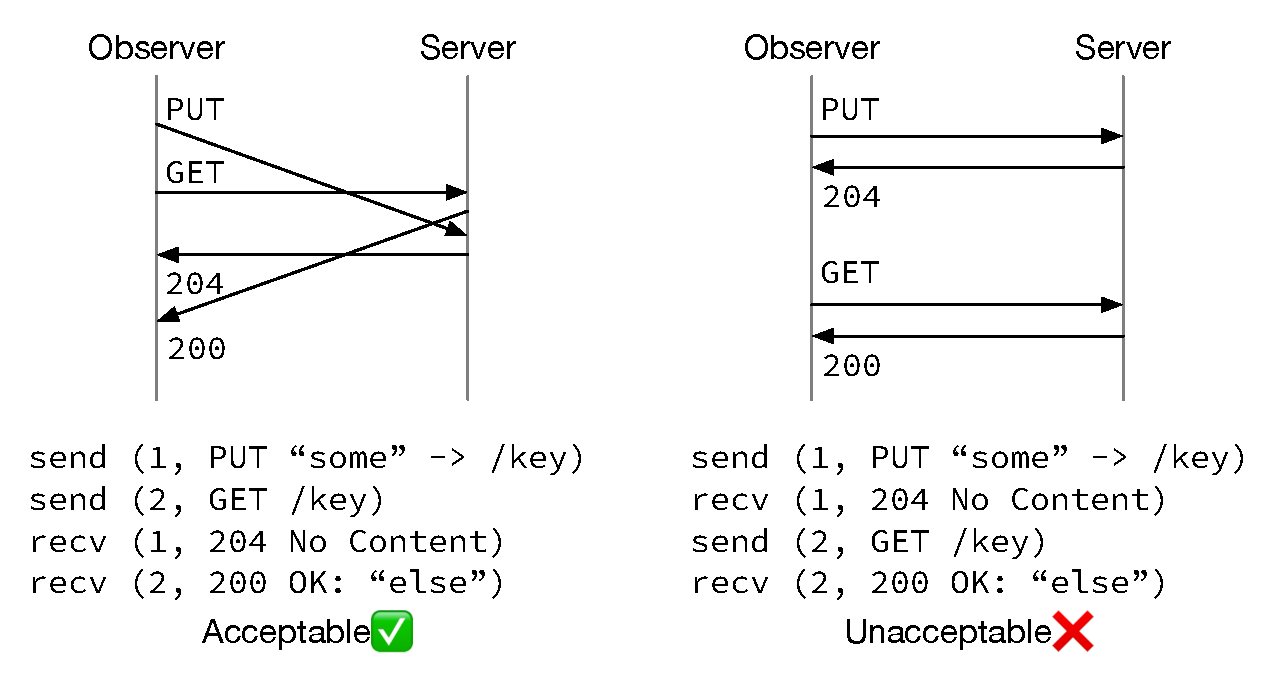
\includegraphics[width=\linewidth]{figures/http-put-bug}
    \caption{The trace on the left does not convince the tester that the server
      is buggy, because there exists a certain network delay that explains why
      the PUT request was not reflected in the 200 response.  When the trace is
      ordered as shown on the right, the tester cannot imagine any network
      reordering that causes such observation, thus must reject the server.}
    \label{fig:put-bug}
  \end{figure}
  \item Mutants 19 and 20 are related to the WebDAV module, which handles PUT
    requests that modify the target's contents.  The buggy servers wrote to a
    different target from that requested, but responds a successful status to
    the client.  The tester cannot tell that the server is faulty until it
    queries the target's latest contents and observes an unexpected value.  To
    reject the server with full confidence, these observations must be made in a
    certain order, as shown in \autoref{fig:put-bug}.

  \item Mutant 18 is similar to the bug in vanilla Apache: the server should have
    responded with 304 Not Modified, but sent back 200 OK instead.  To reveal
    such violation, a minimal counterexample consists of 4 messages: (1) GET
    request, (2) 200 OK response with some ETag \inlinec{x}, (3) GET request
    conditioned over \inlinec{If-None-Match: x}, and (4) 200 OK response,
    indicating that the ETag \inlinec{x} did not match itself.  Notice that (2) must be
    observed before (3), otherwise the tester will not reject the server, with a
    similar reason as \autoref{fig:put-bug}.

  \item Mutant 5 causes the server to skip some code in the core module, and
    send nonscence messages when it should respond with 404 Not Found.  The
    counterexample can be as small as one GET request on a non-existential
    target, followed by a non-404, non-200 response.  However, our tester
    generates request targets within a small range, so the requests' targets are
    likely to be created by the tester's previous PUT requests.  Narrowing the
    range of test case generation might improve the performance in
    aforementioned Mutants 18--20, but Mutant 5 shows that it could
    also degrade the performance of finding some bugs.

  \item The mutants in proxy module caused the server to forward wrong requests
    or responses.  When the origin server part of the tester accepts a
    connection from the proxy, it does not know for which client the proxy is
    forwarding requests.  Therefore, the tester needs to check the requests sent
    by all clients, and make sure none of them matches the incoming proxy
    request, before rejecting the proxy.
\end{itemize}

These examples show that the time-consuming issue of some mutants are likely
caused by limitations in the test case generators.  Cases like Mutant 5 can be
optimized by tuning the request generator based on the tester model's runtime
state, but for Mutants 18--20, the requests should be sent at
specific time periods so that the resulting trace is unacceptable per
specification.  How to produce a specific order of messages is to be explored in
future work.
